\documentclass[11pt]{jabs}
% -- Fonts & Spacing --
\setlength{\parindent}{0pt}
\renewcommand{\baselinestretch}{1.2} % Line spacing
\usepackage{mathptmx}
\usepackage{float}
\usepackage[table]{xcolor}
\pagestyle{plain}

% -- Section Styling --
\titleformat{\section}{\large\bfseries}{\thesection}{1em}{}
\titleformat{\subsection}{\normalsize\bfseries}{\thesubsection}{1em}{}
\titlespacing*{\section}{0pt}{1.25em}{1em}
\titlespacing*{\subsection}{0pt}{1em}{0.5em}

% -- Abstract Box Styling --
\tcbset{
  colback=gray!10,
  colframe=black,
  width=\textwidth,
  arc=2mm,
  boxrule=0.4pt,
  left=6pt, right=6pt, top=6pt, bottom=6pt,
  boxsep=5pt,
}

% -- Custom Colors --
\definecolor{leftbarcolor}{HTML}{F2F2F2}
\definecolor{jabsgreen}{HTML}{00713D}

% -- Custom Box for Metadata Left Panel --
\newmdenv[
  backgroundcolor=leftbarcolor,
  linecolor=white,
  innerleftmargin=8pt,
  innerrightmargin=8pt,
  innertopmargin=10pt,
  innerbottommargin=10pt,
  roundcorner=2pt
]{leftinfobox}

% -- Hyperref Link Colors --
\hypersetup{
    colorlinks=true,
    linkcolor=blue,
    urlcolor=blue,
    citecolor=blue,
}

\usepackage{fancyhdr}
\usepackage{lipsum} 
\usepackage{hyperref}
\usepackage{xcolor}
\usepackage{fontawesome5}
\usepackage{float}


\definecolor{jabsgreen}{RGB}{0,128,0} % green color

% TITLE PAGE style 
\fancypagestyle{titlepagestyle}{
  \fancyhf{}
  \fancyfoot[C]{\small
    JABS 2025 \textbar{} 
    \href{https://doi.org/10.53974/unza.jabs.8.4.1405}{https://doi.org/10.53974/unza.jabs.8.4.1405}
  }
  \renewcommand{\headrulewidth}{0pt}
  \renewcommand{\footrulewidth}{0.4pt}
}

% MAIN style - header + footer with page number and DOI
\fancypagestyle{mainstyle}{
  \fancyhf{}
  \fancyhead[L]{\textit{Journal of Agriculture and Biomedical Sciences -- JABS 2024}}
  \fancyhead[R]{\textbar{} Volume 8 \textbar{} Issue 4}
  \fancyfoot[C]{\small
    JABS 2025 \textbar{} 
    \href{https://doi.org/10.53974/unza.jabs.8.4.1405}{https://doi.org/10.53974/unza.jabs.8.4.1405}
  }
  \fancyfoot[R]{\thepage}
  \renewcommand{\headrulewidth}{0.4pt}
  \renewcommand{\footrulewidth}{0.4pt}
}

\begin{document}

\vspace*{-1in} % Adjust negative space if needed

\pagestyle{titlepagestyle} % apply footer with DOI

\noindent
\begin{minipage}{\textwidth}

  % Logos row
  \noindent
  \begin{minipage}[c]{0.25\textwidth}
    
\includegraphics[width=2\linewidth,height=3cm,keepaspectratio]{images/logo-left.png}
  \end{minipage}%
  \hfill
  \begin{minipage}[c]{0.5\textwidth}
    \centering
    \textit{\makebox[0pt][c]{Journal of Agriculture and Biomedical Sciences -- JABS 2024}}
  \end{minipage}%
  \hfill
  \begin{minipage}[c]{0.25\textwidth}
    \raggedleft
    
\includegraphics[width=2\linewidth,height=3cm,keepaspectratio]{images/logo-right.png}
  \end{minipage}

  \vspace{0.5em}
  {\color{jabsgreen}\rule{\textwidth}{2pt}}
  \vspace{1em}

  % Metadata + abstract content row
  \noindent
  \begin{minipage}[t]{0.35\textwidth}
    \begin{leftinfobox}
      \small
      \href{https://example.com}{
\includegraphics[width=0.9\linewidth]{images/check_for_updates.png}}\\[0.5em]
      \faUnlock \textbf{~OPEN ACCESS} \\[0.75em]
      \textbf{How to Cite:} \\
      John Doe, Jane Doe J, Doe J, John. Optimization of the production of a JABS journal in LaTeX \\
      \textit{Journal of Agricultural and Biomedical Sciences}. 8(4). \\
      \url{https://journals.unza.zm/index.php/JABS/article/view/1405} \\[1em]

      \textbf{Published:} 25\textsuperscript{th} May 2025 \\[0.5em]

      \textbf{Copyright:} \\
      {\small\faCopyright} This is an open access article distributed under the terms of the \\
      \href{https://creativecommons.org/licenses/by/4.0/}{Creative Commons Attribution License}, which permits unrestricted use, distribution, and reproduction in any medium, provided the original author and source are credited. \\[0.5em]

      \textbf{Competing interests:} \\
      The authors declare no conflict of interest.
    \end{leftinfobox}
  \end{minipage}%
  \hfill
  \begin{minipage}[t]{0.62\textwidth}
    \vspace{0pt}
    \textbf{RESEARCH ARTICLE} \\[0.6em]

    {\Large\bfseries [INSERT TITLE HERE]} \\[1em]

    \small
    \textbf{Author one \textsuperscript{1,2*}, Author two\textsuperscript{1}, Author three\textsuperscript{3}, Author Four\textsuperscript{1}} \\[0.5em]

    \textsuperscript{1}Department of Food Science and Nutrition, School of Agricultural Sciences, University of Zambia, Lusaka \\
    \textsuperscript{2}National Institute for Scientific and Industrial Research, Lusaka, Zambia \\
    \textsuperscript{3}Zambia Agricultural Research Institute, Chilanga, Zambia \\[0.5em]

    \textbf{* Corresponding author:} \href{mailto:yourmail@hotmail.com}{yourmail@hotmail.com} / \href{mailto:yourmail@nisir.org.zm}{yourmail@nisir.org.zm}

    \vspace{1em}
    \normalsize
    \textbf{Abstract} \\[0.25em]
    \justifying
    \sloppy
    Lorem ipsum dolor sit amet, consectetuer adipiscing elit. Ut
  purus elit, vestibulum ut, placerat ac, adipiscing vitae, felis.
  Curabitur dictum gravida mauris. Nam arcu libero, nonummy
  eget, consectetuer id, vulputate a, magna. Donec vehicula
  augue eu neque. Pellentesque habitant morbi tristique senec-
  tus et netus et malesuada fames ac turpis egestas. Mauris ut
  leo. Cras viverra metus rhoncus sem. Nulla et lectus vestibu-
  lum urna fringilla ultrices. Phasellus eu tellus sit amet tortor
  gravida placerat.

    \vspace{1em}
    \textbf{Keywords:} Keyword1, Keyword2, Keyword3.
  \end{minipage}

\end{minipage}

\clearpage

% Switch to main page style and start page numbering
\pagestyle{mainstyle}
\setcounter{page}{1}
\pagenumbering{arabic}
\switchcolumn

\begin{adjustwidth}{0.35\textwidth}{0pt} % shift content right by 35% of the page width% --- Main content starts here ---

\section*{Introduction}
\lipsum[1-2]

\section*{Materials and Methods}
\lipsum[3-4]


% Exit adjusted width so image spans full page
\end{adjustwidth}

\vspace{1em}
\begin{figure}[H]
  \centering
  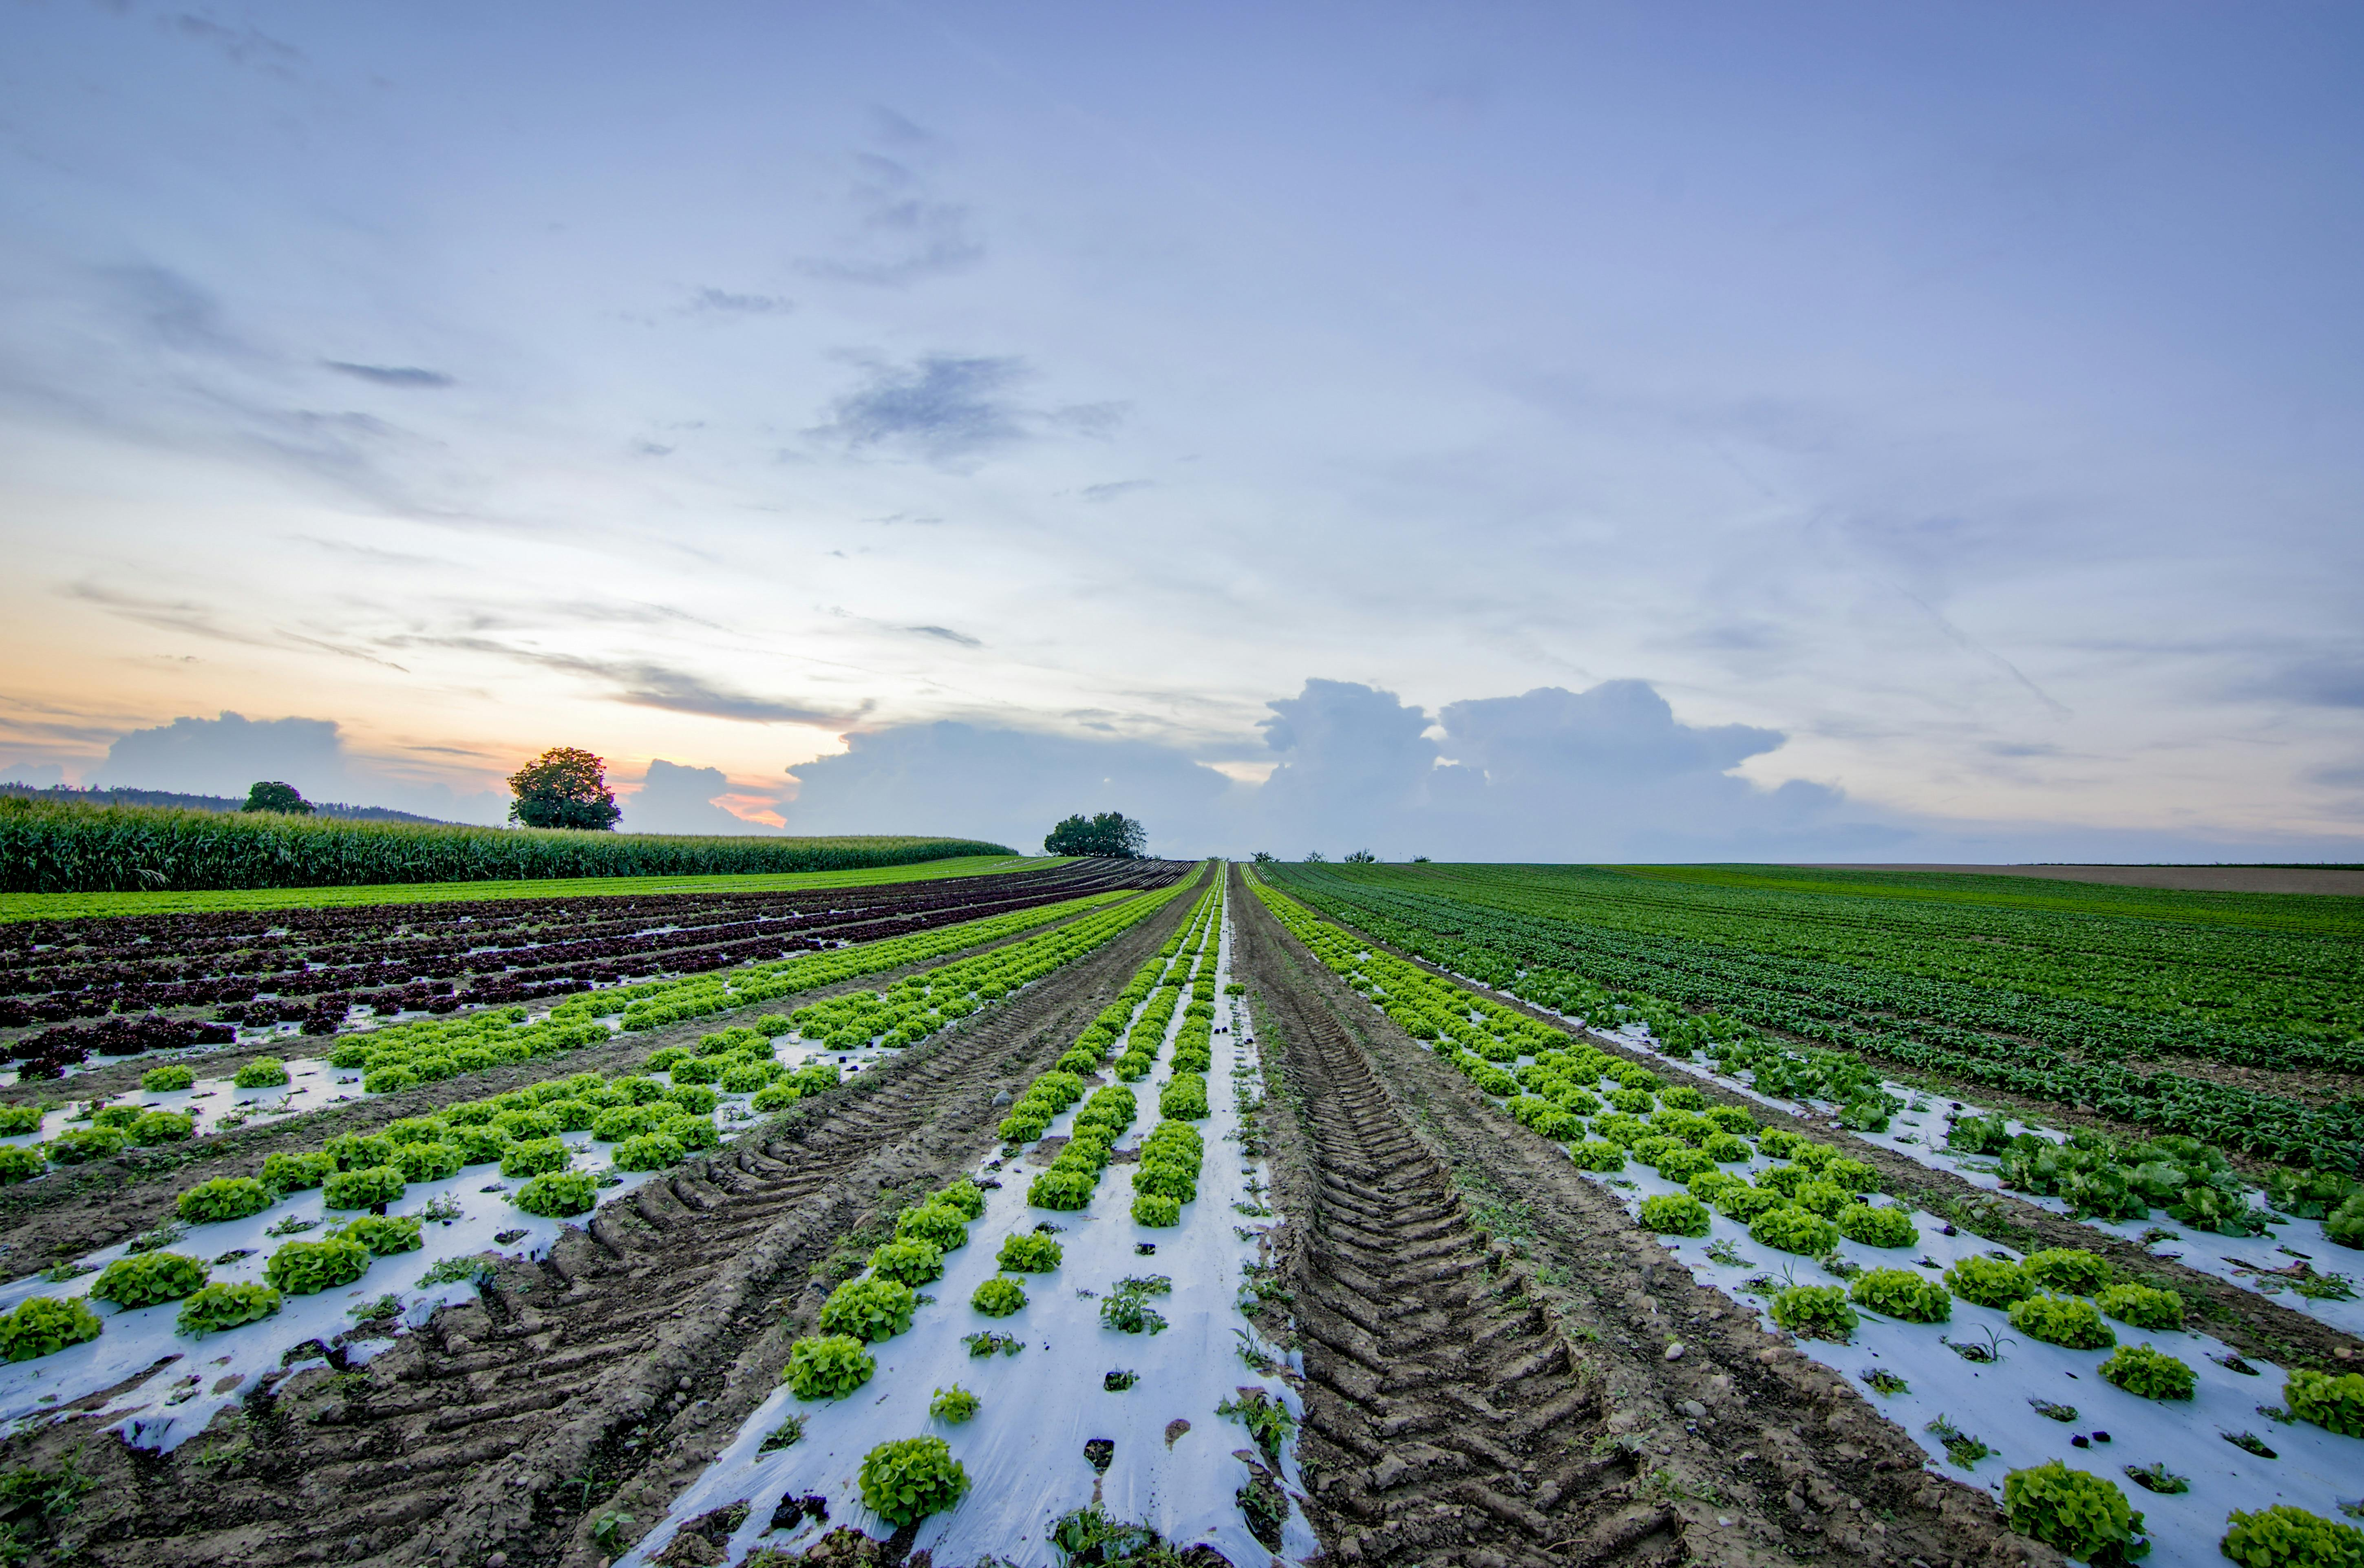
\includegraphics[width=0.7\textwidth]{images/materials-figure.png}
  \caption{Illustration or graphical summary of key findings discussed in the text.}
  \label{fig:materials and methods}
\end{figure}
\vspace{1em}

% Resume adjusted width for rest of text
\begin{adjustwidth}{0.35\textwidth}{0pt}

\section*{Results}
\lipsum[5-6]


% END adjustwidth to allow table to span full page width
\end{adjustwidth}

\vspace{1em}
\rowcolors{2}{gray!10}{white} % alternate row colors starting from second row
\begin{table}[H]
\centering
\renewcommand{\arraystretch}{1.3}
\setlength{\tabcolsep}{12pt}

\begin{tabular}{>{\bfseries}l c c c}
\toprule
Parameter & Group A & Group B & Difference \\
\midrule
Height (cm)      & 165.2 ± 5.1  & 170.8 ± 4.8  & +5.6 \\
Weight (kg)      & 60.3 ± 6.0   & 65.5 ± 5.9   & +5.2 \\
Blood Pressure   & 120/80       & 130/85       & —    \\
Heart Rate (bpm) & 72           & 76           & +4   \\
\bottomrule
\end{tabular}
\caption{\textbf{Comparison of physical and health-related parameters} between Group A and Group B. Values represent mean ± standard deviation.}
\label{tab:styled-results}
\end{table}
\vspace{1em}

\begin{adjustwidth}{0.35\textwidth}{0pt}
\section*{Discussion}
\lipsum[7-8]

\end{adjustwidth}

\vspace{1em}
\begin{figure}[H]
  \centering
  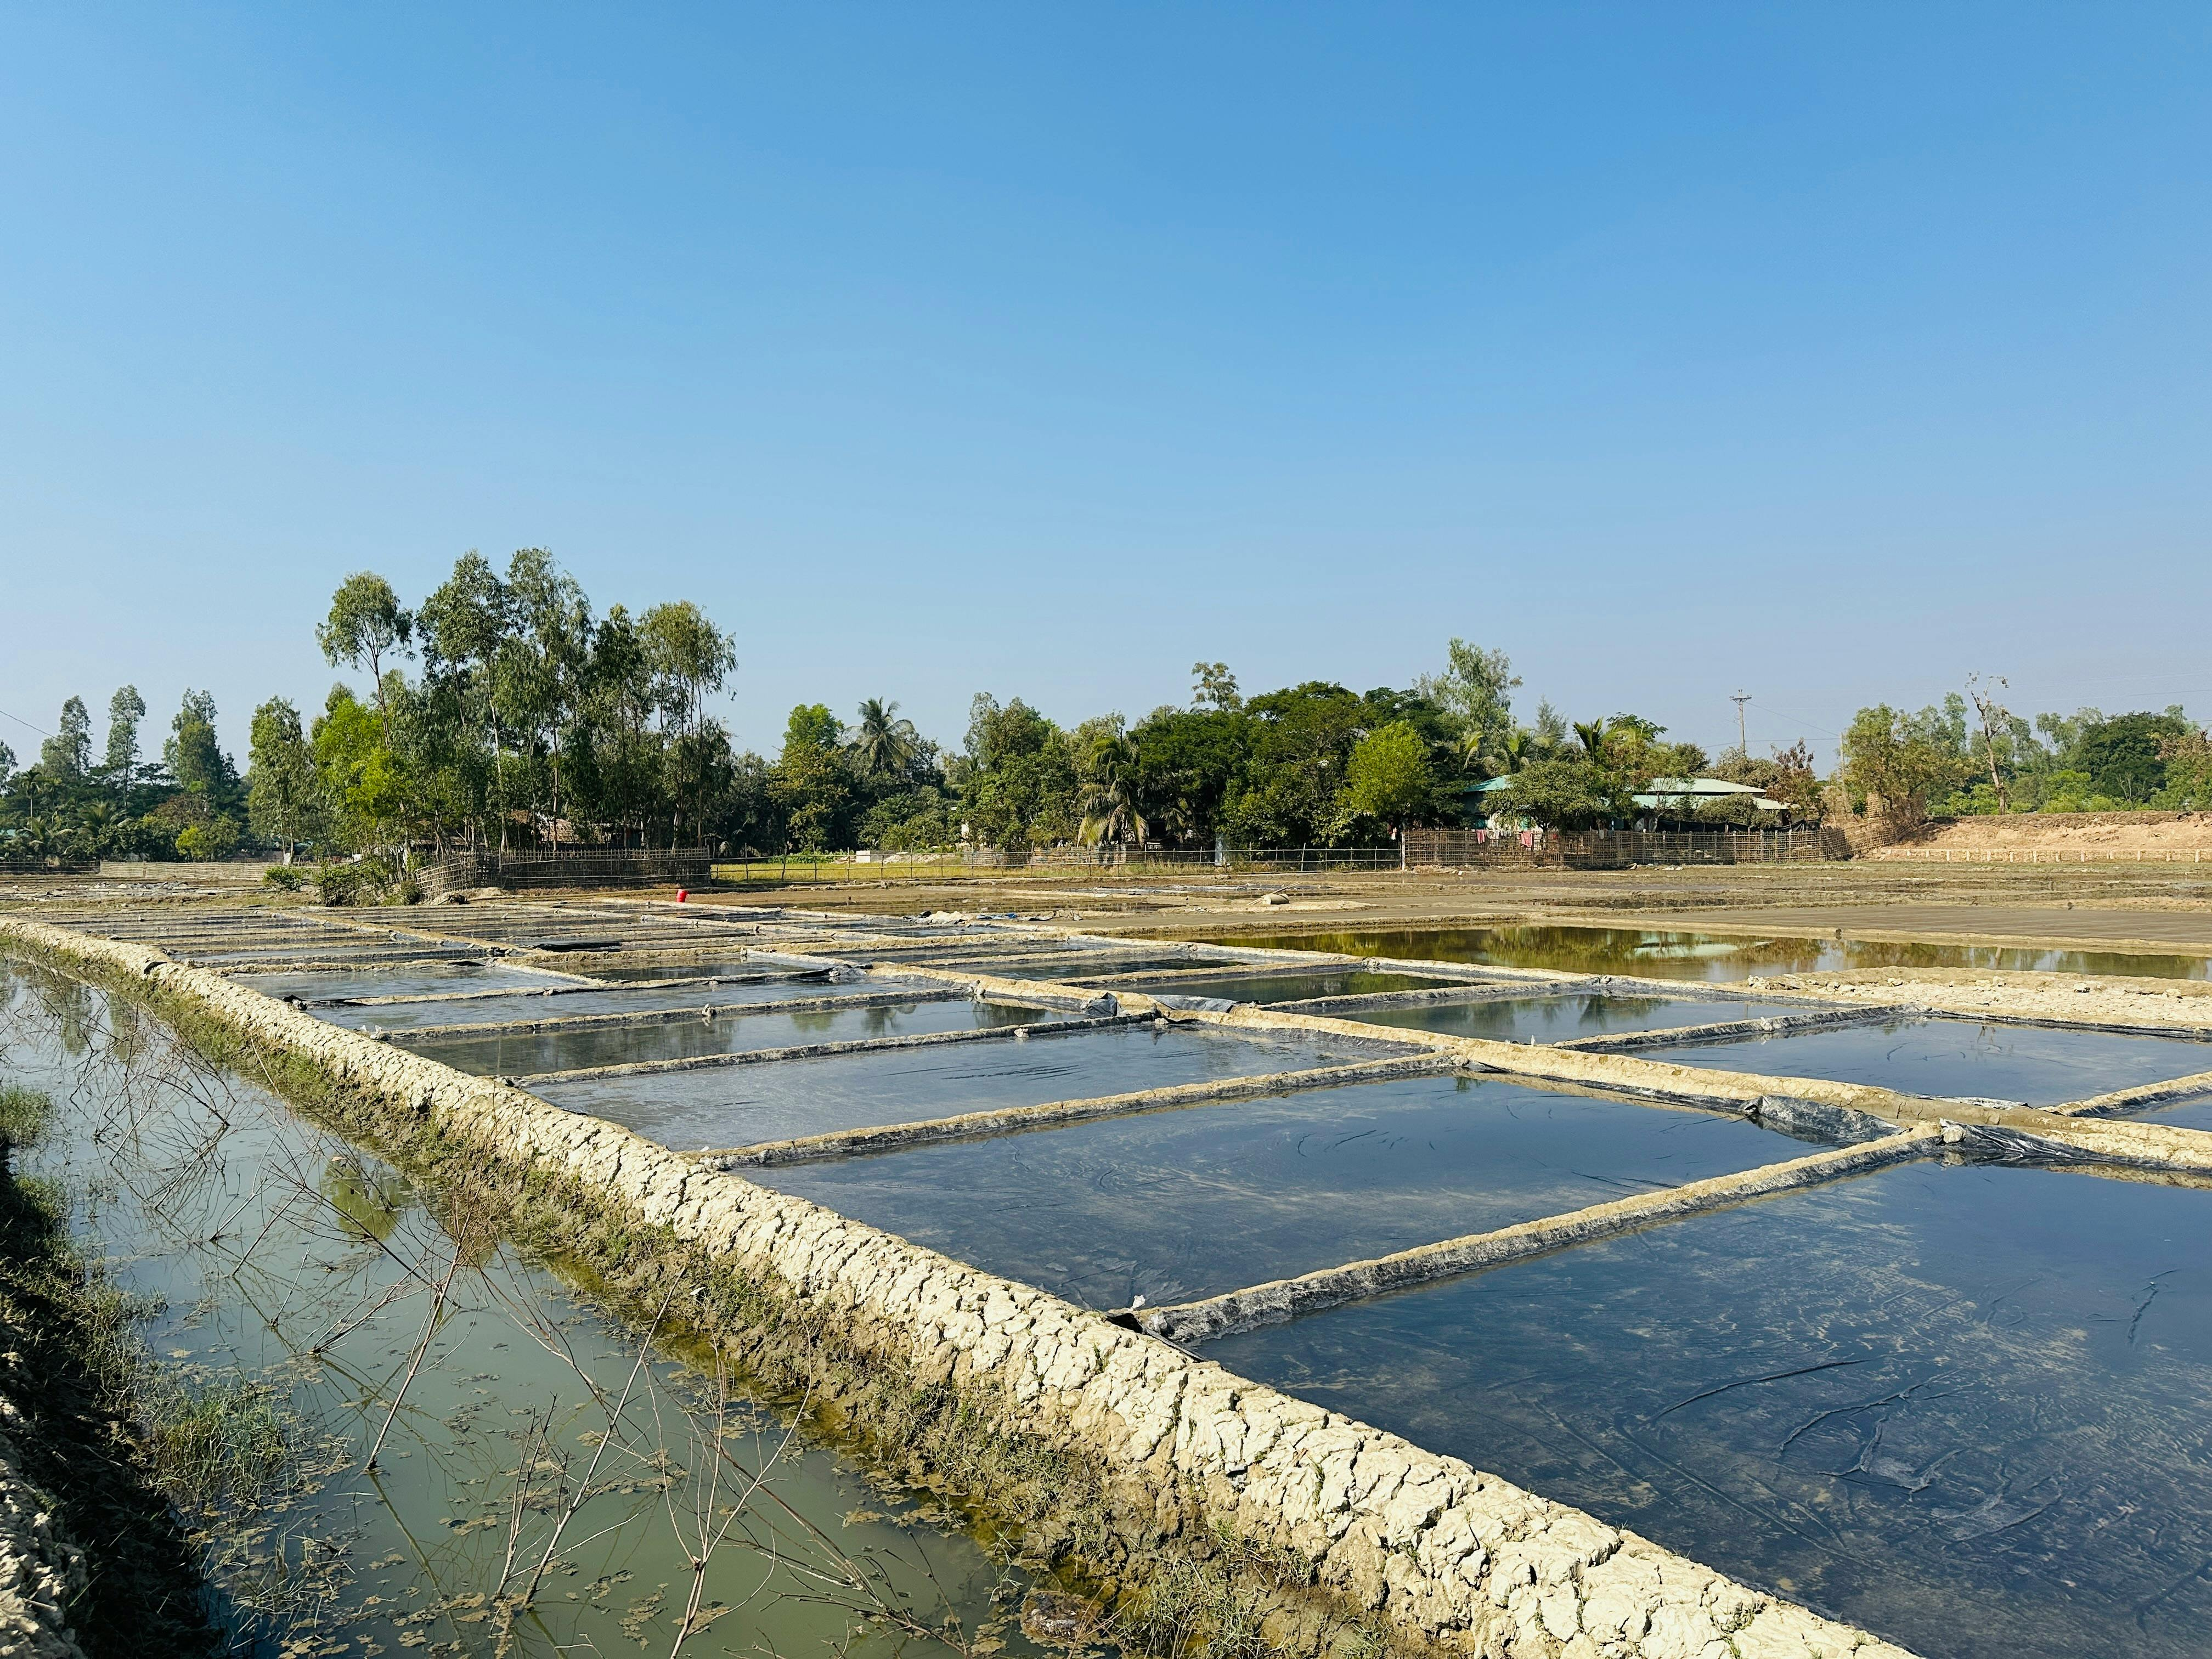
\includegraphics[width=0.7\textwidth]{images/discussion-figure.png}
  \caption{Illustration or graphical summary of key findings discussed in the text.}
  \label{fig:discussion}
\end{figure}
\vspace{1em}

\section*{Acknowledgement}
We thank all contributors and funding sources...

\section*{}
\begin{thebibliography}{9}
\bibitem{ref1} Doe J John.,Jane Doe., et al. (2025). Title of referenced article. \textit{Journal Name}, 8(4), 123–130.
\bibitem{ref2} Another reference...
\end{thebibliography}

\end{adjustwidth}
\end{document}
